\documentclass{article}
\usepackage[sc]{mathpazo}
\linespread{1.15}  
% \usepackage[T1]{fontenc}
%\usepackage[T1]{fontenc}
%\usepackage[sfdefault,scaled=.85]{FiraSans}
%\usepackage{newtxsf}
%\usepackage{mathptmx}
%\usepackage[T1]{fontenc}
%\usepackage{sansmathfonts} 
%\renewcommand*\familydefault{\sfdefault} %% Only if the base font of the document is to be sans serif  
\usepackage[utf8]{inputenc}
\usepackage[margin=2cm]{geometry}
\usepackage{fullpage,enumitem,amssymb,amsmath,tikz,pgfplots,xcolor,cancel,gensymb,hyperref,graphicx,physics,tcolorbox}
\usepackage{indentfirst}
\setlength{\parindent}{0em}
\graphicspath{{./images/}}

\title{Solutions for HW9}
\author{Chris Wang}
\date{\today}

\begin{document}
\maketitle

\begin{tcolorbox}[colframe=blue!50!black, arc=2mm, title=\textsc{Practice 1}]
	\begin{enumerate}[label=(\alph*)]
		\item Intuitively explain why, if we double the wavenumber ($k$) of a wave while keeping the angular frequency ($\omega$) constant, the phase velocity ($|\vec{v}|$) halves. \textit{Think about the definition of angular velocity and how the wavenumber is visually related to wavelength.}
		\item Momentum of a particle is typically given by $p = h / \lambda = \hbar\, k$, where $k$ is the wave number and $\hbar = h / 2\pi$. If the momentum of a particle is doubled, what do you expect happens to its (de Broglie) wavelength? 
	\end{enumerate}
\end{tcolorbox}

\textit{Solution:}

\vspace{1em}

\begin{enumerate}[label=(\alph*)]
    \item Recall that the phase velocity of a wave is 
    \[
    |\vec{v}| = \frac{\omega}{k}.
    \]
    Hence, the velocity is inversely proportional to the wavenumber and proportional linearly to the angular frequency. If we double the wavenumber, we see (based on the animation) that the wavelength halves, so the distance between two crests is also halved. Now, if the angular frequency remains constant, the same time elapses between two crests passing the same point. Hence, if only half the distance is traversed in the same time interval, the phase velocity must be halved.
    \item The equation $p= h / \lambda$ is most useful here. Since $h$ is a constant, doubling the momentum only changes the (de Broglie) wavelength. In this case, the wavelength is halved.
\end{enumerate}

\newpage

\begin{tcolorbox}[colframe=blue!50!black, arc=2mm, title=\textsc{Practice 2}]
	The A string on a cello produces a fundamental frequency of 220 Hz. If I gently put my finger somewhere on the string, I can generate an ethereal 880 Hz sound. If the length of the string is $L$, where on the string am I putting my finger? (\textit{Hint: think about the boundary conditions of the string and which of the harmonics satisfy these boundary conditions. There are two possible answers.})
\end{tcolorbox}

\textit{Solution:}

\vspace{1em}

The cello string is a case where both ends are fixed; hence, they are nodes. In that case, 220 Hz corresponds to half a cycle (the fundamental frequency). By putting my finger on the string, I essentially induce another node somewhere along the string that forces the new ``fundamental frequency'' to be 880 Hz. In essence, the node provides a boundary condition that the new wave must satisfy. We can see a figure that illustrates this below:

\vspace{1cm}

\begin{figure}[h!]
    \centering
    \begin{minipage}{0.4\textwidth}
        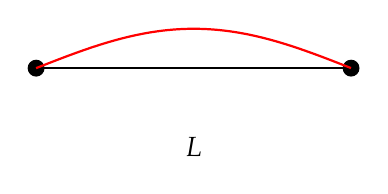
\begin{tikzpicture}[domain=-2:2, samples=100]
            \draw[-, thick] (-2,0) -- (2,0);
            \draw[fill=black] (-2,0) circle (0.1cm);
            \draw[fill=black] (2,0) circle (0.1cm);
            \node at (0,-1) {$L$};
            \draw[color=red,thick] plot(\x, {0.5*sin(0.785 * (\x+2)  r)});
        \end{tikzpicture}
    \end{minipage}
    \hfill
    \begin{minipage}{0.4\textwidth}
        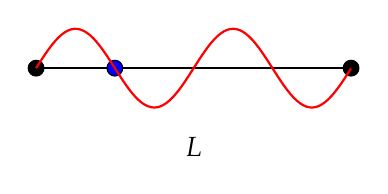
\begin{tikzpicture}[domain=-2:2, samples=100]
            \draw[-, thick] (-2,0) -- (2,0);
            \draw[fill=black] (-2,0) circle (0.1cm);
            \draw[fill=black] (2,0) circle (0.1cm);
            \draw[fill=blue] (-1,0) circle (0.1cm);
            \draw[color=red,thick] plot(\x, {0.5*sin(3.14 * (\x+2)  r)});
            \node at (0,-1) {$L$};
        \end{tikzpicture}
    \end{minipage}
    \caption{On the left: The fundamental frequency of the string. On the right: The new ``fundamental frequency'' once my finger is placed on the string.}
\end{figure}

\vspace{1em}

We also observe that the new frequency is four times the original fundamental frequency, which implies that the new wavelength is a quarter of the original wavelength. Hence, the finger is placed at $L/4$ or $3L/4$.

\newpage

\begin{tcolorbox}[colframe=blue!50!black, arc=2mm, title=\textsc{Practice 3}]
	The reason I brought up Taylor series here is because the Rayleigh criterion mentioned in Q3 relates the diffraction limit of an aperture to the wavelength of light and the aperture size \textit{nonlinearly}. The nonlinear nature can make calculations annoying, especially at smaller angular separations. The Rayleigh criterion is given by
	\[
		\sin \theta = 1.22 \frac{\lambda}{D},
	\]
	where $\theta$ is the angular separation between two objects of interest, $\lambda$ is the wavelength of light, and $D$ is the diameter of the aperture.
	\begin{enumerate}[label=(\alph*)]
		\item Taylor expand $\sin \theta$ about $\theta = 0$ to first order and find the minimum aperture diameter $D$ that can resolve two objects separated by $\theta = 1$ arcsecond using light of wavelength $\lambda = 500$ nm.
		\item For larger values of $\theta$, truncating the series at first order may be insufficient. Find the next nonzero term in the Taylor series for $\sin\theta$ and compare the error between the series in (a) containing only one term, the new series, and the true value for $\theta=\pi / 4$.
	\end{enumerate} 
\end{tcolorbox}

\textit{Solution:}

\vspace{1em}

\begin{enumerate}[label=(\alph*)]
    \item To first order around $\theta = 0$, the Taylor expansion of $\sin \theta$ is
    \[
    \sin \theta \simeq \sin(0) + \dv{\sin \theta}{\theta} \Big|_{\theta = 0} \theta = 0 + \cos(0) \, \theta = \theta.
    \]
    We can now find $D$ by algebraically isolating the equation above:
    \[
    \theta = 1.22 \frac{\lambda}{D} \quad \implies \quad D = 1.22 \frac{\lambda}{\theta}
    \]
    Note that 1 arcsecond is $1 / (3600*57.3)$ radians. Hence, $D = 1.22 \times 5 \times 10^{-7} / (1 / (3600*57.3)) \approx 0.13$ m.
    \item Let's repeat the above expansion, bringing it further:
    \[
    \sin\theta \simeq \theta + \underbrace{\cancel{\dv[2]{\sin \theta}{\theta} \Big|_{\theta = 0} \, \frac{\theta^2}{2!}}}_{0} + \dv[3]{\sin\theta}{\theta} \Big|_{\theta=0} \, \frac{\theta^3}{3!} = \theta - \frac{\theta^3}{3!}.
    \]
    Let's compare for $\theta = \pi / 4$:
    \[
    \sin(\pi / 4) = \sqrt{2} / 2 \approx 0.7071, \quad \theta = \pi / 4 \approx 0.7854, \quad \theta - \frac{\theta^3}{3!} \approx 0.7046.
    \]
    Evidently, adding in next term in the expansion greatly improves its accuracy, even for relatively larger angular displacements away from $\theta=0$.
\end{enumerate}

\newpage

\begin{tcolorbox}[arc=2mm, title=\textsc{The Wave Equation (Enrichment)}]
	While this is not something you need to worry about for now, if you are interested, the form of the wave equation is 
	\[
		\pdv[2]{w}{t} = v^2 \pdv[2]{w}{x},
	\]
	where $w$ describes the wave solution and $v$ is the wave speed. If you are familiar with differential equations and want to try an extra problem, show that the wave function $w(t,x) = A\sin(kx-\omega t) + B\sin(kx+\omega t)$ is a solution to the wave equation.
\end{tcolorbox}

\textit{Solution:}

\vspace{1em}

Plug our trial solution into the wave equation:
\begin{align*}
    \pdv[2]{w}{t} &= -A\omega^2 \sin(kx-\omega t) - B\omega^2 \sin(kx+\omega t) \\
    \pdv[2]{w}{x} &= -Ak^2 \sin(kx-\omega t) - Bk^2 \sin(kx+\omega t) \\
    \text{Observe that since }v^2 = \omega^2 / k^2:& \\
    v^2 \pdv[2]{w}{x} &= -\frac{\omega^2}{k^2}\left( Ak^2\sin(kx-\omega t) + Bk^2 \sin(kx + \omega t) \right) \\
    &= -A\omega^2 \sin(kx-\omega t) - B\omega^2 \sin(kx+\omega t) \\
    &= \pdv[2]{w}{t}.
\end{align*}


\end{document}